\section{Definição da sintaxe}

\begin{frame}[fragile]{Definições}

    \begin{itemize}
        \item Uma gramática deve descrever a estrutura hierárquica de seus elementos
       %\pause

        \item Por exemplo, o comando \texttt{if-else} da linguagem C, possui a forma
            \inputsyntax{c}{codes/if.c}
        a qual pode ser expressa como
        \begin{footnotesize}
        \[
            cmd \to \mathbf{if}\ (expr)\ cmd\ \mathbf{else}\ cmd
        \] 
        \end{footnotesize}%\pause
        \item A expressão acima é uma regra de produção, onde a seta significa ``pode ter a forma''
       %\pause

        \item Os elementos léxicos da produção (palavras-chaves, parêntesis) são chamados tokens ou terminais
       %\pause

        \item Variáveis como $expr$ e  $cmd$ representam sequências de tokens e são denominadas não-terminais
    \end{itemize}

\end{frame}

\begin{frame}[fragile]{Componentes da linguagem livre de contexto}

    \begin{enumerate}
        \item Um conjunto de tokens, denominados símbolos terminais
       %\pause

        \item Um conjunto de não-terminais
       %\pause

        \item Um conjunto de produções. Cada produção é definida por um não-terminal (lado esquerdo), seguido de uma seta, sucedida por uma sequência de tokens
            e/ou não-terminais (lado direito)
       %\pause

        \item Designação de um dos não-terminais como símbolo de partida
    \end{enumerate}

\end{frame}

\begin{frame}[fragile]{Convenções de notação da gramática livre de contexto}

    \begin{itemize}
        \item A gramática é especificada por uma lista de produções
       %\pause

        \item O símbolo de partida é definido como o não-terminal da primera produção listada
       %\pause

        \item Dígitos, símbolos e palavras em negrito são terminais
       %\pause

        \item Não-terminais são grafados em itálico
       %\pause

        \item Os demais símbolos são tokens
       %\pause

        \item Produções distintas de um mesmo não-terminal podem ser agrupadas por meio do caractere \code{cpp}{'|'}, que significa, neste contexto, ``ou''
    \end{itemize}

\end{frame}

\begin{frame}[fragile]{Exemplo de sintaxe para expressões infixas com adição e subtração}

    \begin{itemize}
        \item Considere a seguinte gramática para expressões compostas por dígitos decimais e as operações de adição e subtração, em forma infixa:
    \[
        \begin{array}{rcl}
            expr & \to & expr + digito\ |\ expr - digito\ |\ digito \\
            digito & \to & 0 \ | \  1 \ | \  2 \ | \  3 \ | \  4 \ | \  5 \ | \  6 \ | \  7 \ | \  8 \ | \  9
        \end{array}
    \]
   %\pause

        \item Os tokens desta gramática são os dez dígitos decimais e os caracteres \code{cpp}{'+'} e \code{cpp}{'-'}
       %\pause

        \item Os não-terminais são $expr$ e $digito$
       %\pause

        \item O símbolo de partida é o não-terminal $expr$
    \end{itemize}

\end{frame}

\begin{frame}[fragile]{Cadeias de tokens}

    \begin{itemize}
        \item Uma cadeia de tokens é uma sequência de zero ou mais tokens
       %\pause

        \item Uma cadeia contendo zero tokens, grafada como \code{apl}{∊}, é denominada cadeia vazia
       %\pause

        \item Uma gramática deriva cadeias de tokens começando pelo símbolo de partida, substituíndo repetidamente um não-terminal pelo lado direito de uma
            produção deste não-terminal
       %\pause

        \item O conjunto de todas as cadeias de tokens possíveis gerados desta maneira formam a linguagem definida pela gramática
    \end{itemize}

\end{frame}

\begin{frame}[fragile]{Exemplo de construção da expressão \code{cpp}{1-2+3} por meio da gramática}

    \begin{enumerate}
        \item \code{cpp}{1} é $expr$, pois \code{cpp}{1} é $digito$ (terceira alternativa para a produção de $expr$)
       %\pause

        \item Pela segunda alternativa de produção de $expr$,  \code{cpp}{1-2} é também $expr$, pois \code{cpp}{1} é $expr$ e \code{cpp}{2} é $digito$
       %\pause

        \item Por fim, pela primeira alternativa de produção de $expr$, \code{cpp}{1-2+3} é $expr$, pois \code{cpp}{1-2} é $expr$ e \code{cpp}{3} é $digito$
    \end{enumerate}

\end{frame}

\begin{frame}[fragile]{Árvore gramatical}

    Dada uma gramática livre de contexto, uma árvore gramatical possui as seguintes propriedades:
   %\pause

    \begin{enumerate}
        \item A raiz é rotulada pelo símbolo de partida
       %\pause

        \item Cada folha é rotulada por um token ou por \code{apl}{∊}
       %\pause

        \item Cada nó interior é rotulado por um não-terminal
       %\pause

        \item Se $A$ é um não-terminal que rotula um nó interior e $X_1, X_2, \ldots, X_N$ são os rótulos de seus filhos (da esquerda para a direita), então
        \[
            A \to X_1\ X_2\ \ldots X_N
        \]
        é uma produção
    \end{enumerate}

\end{frame}

\begin{frame}[fragile]{Visualização da árvore gramatical da expressão \code{cpp}{1-2+3}}

    \begin{figure}
        \centering

        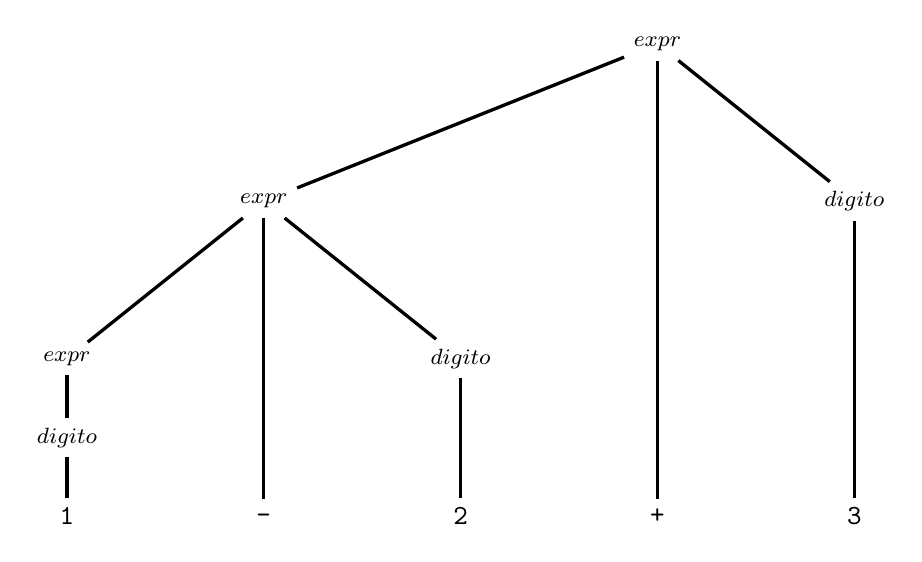
\begin{tikzpicture} 
            \node (A) at (0, 0) { \texttt{1} };
            \node (B) at (0, 1) { \footnotesize $digito$ };
            \node (C) at (0, 2) { \footnotesize $expr$ };
            \node (D) at (2.5, 0) { \texttt{-} };
            \node (E) at (2.5, 4) { \footnotesize $expr$ };
            \node (F) at (5, 0) { \texttt{2} };
            \node (G) at (5, 2) { \footnotesize $digito$ };
            \node (H) at (7.5, 6) { \footnotesize $expr$ };
            \node (I) at (7.5, 0) { \texttt{+} };
            \node (J) at (10, 4) { \footnotesize $digito$ };
            \node (K) at (10, 0) { \texttt{3} };

            \draw[very thick] (A) to (B);
            \draw[very thick] (C) to (B);
            \draw[very thick] (C) to (E);
            \draw[very thick] (E) to (D);
            \draw[very thick] (F) to (G);
            \draw[very thick] (E) to (G);
            \draw[very thick] (E) to (H);
            \draw[very thick] (I) to (H);
            \draw[very thick] (H) to (J);
            \draw[very thick] (K) to (J);
        \end{tikzpicture} 
    \end{figure}

\end{frame}

\begin{frame}[fragile]{Características da árvore gramatical}

    \begin{itemize}
        \item As folhas da árvore gramatical, quando lidas da esquerda para a direita, formam o produto da árvore, que é a cadeira gerada ou derivada a partir
            da raiz não-terminal
           %\pause

        \item O processo de encontrar uma árvore gramatical para uma dada cadeia de tokens é chmado de análise gramatical ou análise sintática daquela cadeia
       %\pause

        \item Uma gramática que permite a construção de duas ou mais árvores gramaticais distintas para uma mesma cadeia de tokens é denominada gramática
            ambígua
       %\pause

        \item A gramatica apresentada não é ambígua
       %\pause

        \item Contudo, se removida a distinção entre $expr$ e $digito$, a gramática passaria a ser ambígua:
        \begin{footnotesize}
        \[
            expr \to expr + expr\ |\ expr - expr\ |\ 0 \ | \  1 \ | \  2 \ | \  3 \ | \  4 \ | \  5 \ | \  6 \ | \  7 \ | \  8 \ | \  9
        \]
        \end{footnotesize}
    \end{itemize}

\end{frame}

\begin{frame}[fragile]{Exemplo de gramática ambígua}

    \begin{figure}
        \centering

        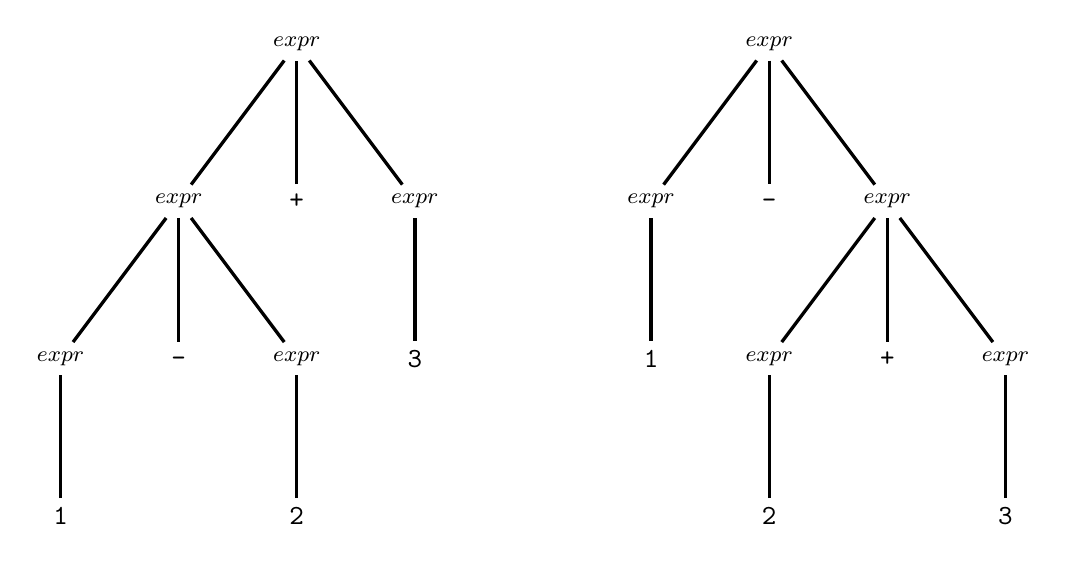
\begin{tikzpicture} 
            \node (A) at (0, 0) { \texttt{1} };
            \node (C) at (0, 2) { \footnotesize $expr$ };
            \node (D) at (1.5, 2) { \texttt{-} };
            \node (E) at (1.5, 4) { \footnotesize $expr$ };
            \node (F) at (3, 0) { \texttt{2} };
            \node (G) at (3, 2) { \footnotesize $expr$ };
            \node (H) at (3, 6) { \footnotesize $expr$ };
            \node (I) at (3, 4) { \texttt{+} };
            \node (J) at (4.5, 4) { \footnotesize $expr$ };
            \node (K) at (4.5, 2) { \texttt{3} };

            \draw[very thick] (A) to (C);
            \draw[very thick] (C) to (E);
            \draw[very thick] (E) to (D);
            \draw[very thick] (F) to (G);
            \draw[very thick] (E) to (G);
            \draw[very thick] (E) to (H);
            \draw[very thick] (I) to (H);
            \draw[very thick] (H) to (J);
            \draw[very thick] (K) to (J);

            \node (A1) at (7.5, 2) { \texttt{1} };
            \node (C1) at (7.5, 4) { \footnotesize $expr$ };
            \node (D1) at (9, 4) { \texttt{-} };
            \node (E1) at (9, 6) { \footnotesize $expr$ };
            \node (F1) at (9, 0) { \texttt{2} };
            \node (G1) at (9, 2) { \footnotesize $expr$ };
            \node (H1) at (10.5, 4) { \footnotesize $expr$ };
            \node (I1) at (10.5, 2) { \texttt{+} };
            \node (J1) at (12, 2) { \footnotesize $expr$ };
            \node (K1) at (12, 0) { \texttt{3} };

            \draw[very thick] (A1) to (C1);
            \draw[very thick] (C1) to (E1);
            \draw[very thick] (E1) to (D1);
            \draw[very thick] (F1) to (G1);
            \draw[very thick] (E1) to (H1);
            \draw[very thick] (I1) to (H1);
            \draw[very thick] (H1) to (J1);
            \draw[very thick] (H1) to (G1);
            \draw[very thick] (K1) to (J1);
        \end{tikzpicture} 
    \end{figure}

\end{frame}

\begin{frame}[fragile]{Associatividade de operadores}

    \begin{itemize}
        \item Quando um operando está, simultaneamente, à esquerda e à direita de dois operadores (por exemplo, o dígito \code{cpp}{2} na expressão
            \code{cpp}{1-2+3}), é preciso decidir qual destes operadores receberá o operando
       %\pause

        \item Uma operação $\odot$ é associativa à esquerda se $a\odot b\odot c = (a\odot b)\odot c$
       %\pause

        \item Na maioria das linguagens de programação, os operadores aritméticos (\code{cpp}{+, -, *} e \code{cpp}{/}) são associativos à esquerda
       %\pause

        \item Uma operação $\oslash$ é associativa à direita se $a\oslash b\oslash c = a\oslash (b\oslash c)$
       %\pause

        \item Por exemplo, a atribuição (operador \code{cpp}{=}) da linguagem C é associativa à direita: a expressão \code{cpp}{a = b = c} equivale a expressão
        \code{cpp}{a = (b = c)}
       %\pause

        \item Uma gramática possivel para esta atribuição seria:
        \begin{footnotesize}
        \[
            \begin{array}{rcl}
                expr & \to & var = expr\ |\ var \\
                var & \to & a\ |\ b\ |\ \ldots \ |\ z
            \end{array}
        \]
        \end{footnotesize}
    \end{itemize}

\end{frame}

\begin{frame}[fragile]{Precedência de operadores}

    \begin{itemize}
        \item Algumas expressões da aritmética contém ambiguidades que não podem ser resolvidas apenas por meio da associatividade
       %\pause

        \item Por exemplo, qual seria o resultada expressão \code{cpp}{1 + 2 * 3}? \code{cpp}{9} ou \code{cpp}{7}?
       %\pause

        \item Dizemos que o operador $\otimes$ tem maior precedência do que o operador $\oplus$ se $\otimes$ captura os operandos antes que $\oplus$ o faça
       %\pause

        \item Na aritmética, a multiplicação e a divisão tem maior precedência do que a adição e a subtração
       %\pause

        \item Se dois operadores tem mesma precedência, a associatividade determina a ordem que as operações serão realizadas
    \end{itemize}

\end{frame}

\begin{frame}[fragile]{Construção de gramáticas com precedência de operadores}

    É possível construir uma gramática com precedência de operadores a partir dos seguintes passos:
   %\pause

    \vspace{0.2in}

    \begin{enumerate}
        \item Construa uma tabela com a associatividade e a precedência dos operadores, em ordem crescente de precedência (operadores com mesma precedência 
            aparecem na mesma linha)
       %\pause
        \begin{footnotesize}
        \[
            \begin{array}{lr}
                \mbox{associatividade à esquerda} & \code{cpp}{+}\ \code{cpp}{-} \\
                \mbox{associatividade à esquerda} & \code{cpp}{*}\ \mintinline{cpp}{/} \\
            \end{array}
        \]
        \end{footnotesize}
       %\pause
       
        \item Crie um não-terminal para cada nível ($expr$ e $termo$) e um não-terminal extra para as unidades básicas da expressão ($fator$)
       %\pause
        \begin{footnotesize}
        \[
            fator \to \mathbf{digito}\ |\ (expr)
        \]
        \end{footnotesize}
 
    \end{enumerate}

\end{frame}

\begin{frame}[fragile]{Construção de gramáticas com precedência de operadores}

    \begin{enumerate}
        \setcounter{enumi}{2}
        \item Defina as produções para o último terminal criado para os níveis a partir dos operadores com maior precedência
       %\pause
        \begin{footnotesize}
        \[
            \begin{array}{rcl}
                termo & \to & termo\ \code{cpp}{*}\ fator \\
                & |\ & termo\ \code{cpp}{/}\ fator \\
                & |\ & fator
            \end{array}
        \]
        \end{footnotesize}
       %\pause
       
        \item Faça o mesmo para os demais operadores, em ordem decrescente de precedência e crescente na lista de terminais criados para os níveis
       %\pause
        \begin{footnotesize}
        \[
            \begin{array}{rcl}
                expr & \to & expr\ \code{cpp}{+}\ termo \\
                & |\ & expr\ \code{cpp}{-}\ termo \\
                & |\ & termo
            \end{array}
        \]
        \end{footnotesize}
       %\pause
    \end{enumerate}

    \vspace{0.1in}

    A presença de parêntesis na definição de $fator$ permite escrever expressões com níveis arbitrários de aninhamento, sendo que os parêntesis tem precedência
    sobre todos os operadores definidos.
    
\end{frame}

